\documentclass[a4paper,11pt]{article}
\usepackage[utf8]{inputenc}
\usepackage[spanish]{babel}
\usepackage{amsmath, amssymb}
\usepackage{graphics, subfigure}
\usepackage{lipsum}
\usepackage{array}
\usepackage{hyperref, url}
\usepackage[top=2.5cm, bottom=2.5cm, left=2.5cm, right=2.5cm]{geometry}
\usepackage{float}
\usepackage{multicol}
\usepackage{enumerate}
\usepackage{color, xcolor}
\usepackage{pgfplots}
\usepackage{wrapfig}

\title {Algoritmo Cu\'antico de Shor}
\date{14 de Junio de 2022}
\author{Miguel Alejandro Asin Barthelemy C511\\Jose Carlos Hern\'andez Pi\~nera C511}

\begin{document}

\begin{titlepage}
    \centering
    {
\includegraphics[width=0.13\textwidth]{logo.png}\par}
    \vspace{1cm}
    {\bfseries\LARGE Universidad de la Habana \par}
    \vspace{1cm}
    {\scshape\Large Facultad de Matem\'atica y Computaci\'on \par}
    \vspace{3cm}
    {\scshape\Huge Algoritmo de factorizaci\'on cu\'antico de Shor \par}
    \vspace{3cm}
    {\itshape\Large Tarea de Curso de Historia de la Computaci\'on \par}
    \vfill
    {\Large Autores: \par}
    {\Large Miguel Alejandro Asin Barthelemy C511 \par}
    {\Large Jos\'e Carlos Hern\'andez Pi\~nera C511 \par}
    \vfill
    {\Large Junio 2022 \par}
\end{titlepage}

\section*{Resumen}
\par Como parte del desarrollo de la computaci\'on cu\'antica, se presenta el estudio del algoritmo de factorizaci\'on cu\'antica de Shor, propuesto por Peter Shor en 1995 como una herramienta cu\'antica para determinar en tiempo polinomial la factorizaci\'on en primos de un n\'umero. Se realiza un breve acercamiento a la vida del desarrollador del algoritmo en correspondencia con los logros alcanzados en el campo de la ciencia en que se desempe\~na. Posteriormente, se da la definici\'on formal del algoritmo cu\'antico y posibles aplicaciones que tendr\'ia en el mundo moderno, muy centrado en el \'ambito de la criptograf\'ia y del futuro de la computaci\'on cu\'antica.\\

\par \textbf{Palabras claves:} computaci\'on, cu\'antica, algoritmo, Shor, criptograf\'ia, factorizaci\'on.

\section*{Abstract}
As part of the development of quantum computing, the study of Shor's quantum factorization algorithm is presented, proposed by Peter Shor in 1995 as a quantum tool to determine the prime factors of a number in polynomial time. A brief approach to the life of the developer of the algorithm is made in correspondence with the achievements in the field of science in which it is carried out. Subsequently, the formal definition of the quantum algorithm and the possible applications they have in the modern world are given, very focused on the field of cryptography and the future of quantum computing.

\section*{\center\itshape\large{Introducci\'on}}
\par En la actualidad, grandes empresas de tecnología como IBM, Microsoft, Intel y Google han estado trabajando en relativo silencio sobre lo que podría convertirse en el futuro de la computación: la computación cuántica.

\par A principios del siglo XX, Planck y Einstein proponen que la luz no es una onda continua (como las ondas de un estanque) sino que está dividida en pequeños paquetes o cuantos. Esta idea, en apariencia simple, servía para resolver un problema llamado la ``catástrofe ultravioleta''; pero a lo largo de los años otros físicos fueron desarrollándola y llegando a conclusiones sorprendentes sobre la materia, dos de las cuales son: la superposición de estados y el entrelazamiento.

\par La idea de computación cuántica surge en 1981, cuando Paul Benioff expuso su teoría para aprovechar las leyes cuánticas en el entorno de la informática. En vez de trabajar a nivel de voltajes eléctricos, se trabaja a nivel de cuanto. Como ya es conocido, en la computación clásica la unidad básica de información es el bit, que puede tener dos estados posibles ($1$ o $0$) y con los que es posible realizar varias operaciones lógicas (AND, NOT, OR). Juntando $n$ bits se pueden representar números y operar sobre estos, pero con limitaciones: sólo pueden representarse hasta $2^n$ estados distintos, y si se quiere cambiar un conjunto de estos bits se debe que realizar al menos un igual número de operaciones sobre ellos: no hay forma de cambiarlos mágicamente sin tocarlos. En cambio, en la computación cuántica intervienen las leyes de la mecánica cuántica, y la partícula puede estar en superposición coherente: puede ser $0$, $1$ y puede ser $1$ y $0$ a la vez (dos estados ortogonales de una partícula subatómica). Eso permite que se puedan realizar varias operaciones a la vez, según el número de cúbits.

\par Un claro ejemplo de lo anterior, son los diferentes algoritmos cuánticos que se han desarrollado gracias al entrelazamiento, como lo es el que será objeto de análisis de la presente investigación: el algoritmo de Shor. El algoritmo de Shor es un procedimiento propuesto y desarrollado por Peter Shor en 1995 que permite encontrar factores de un número de una manera eficiente. Primeramente, se brindará un breve panoráma histórico del nacimiento de este algoritmo y de su creador en correspondencia con una definición formal del mismo; y, posteriormente, se analizar\'a el impacto que tiene y pueda tener en la actualidad cient\'ifica (pues este es un tema a\'un joven).

\section*{\center\itshape\large{Peter Shor (1959 - actualidad)}}

\par Peter Williston Shor\textsuperscript{\textcolor{cyan}{\cite{1}}} naci\'o el 14 de agosto de 1959, en New York City, New York. Mientras asistía a la Escuela Secundaria Tamalpais, en Mill Valley, California, ocupó el tercer lugar en la Olimpiada Matemática de EE.UU. de 1977. Después de graduarse ese año, ganó una medalla de plata en la Olimpiada Internacional de Matemáticas en Yugoslavia. Recibi\'o su B.S. en Matemáticas en 1981 para trabajos de pregrado en Caltech, y fue becario de Putnam en 1978. Obtuvo su Ph.D. en Matemáticas Aplicadas del MIT en 1985. Su asesor de doctorado fue F. Thomson Leighton, y su tesis versó sobre el análisis probabilístico de algoritmos de empaque de contenedores.

\par Después de recibir su Ph.D. por el MIT, pasó un año como investigador postdoctoral en la Universidad de California, Berkeley, y luego aceptó un puesto en Bell Labs en New Providence, Nueva Jersey. Fue allí donde desarrolló el algoritmo de Shor, por el que recibió el Premio Nevanlinna en el 23º Congreso Internacional de Matemáticos en 1998 y el Premio Gödel en 1999. En 1999 recibió una beca MacArthur. En 2017 recibi\'o la Medalla Dirac del ICTP (Figura 1) y para 2019 el Premio Fundación BBVA Fronteras del Conocimiento en Ciencias Básicas.

\begin{wrapfigure}{r}{0.3\textwidth}
    \vspace{-20pt}
    \begin{center}
        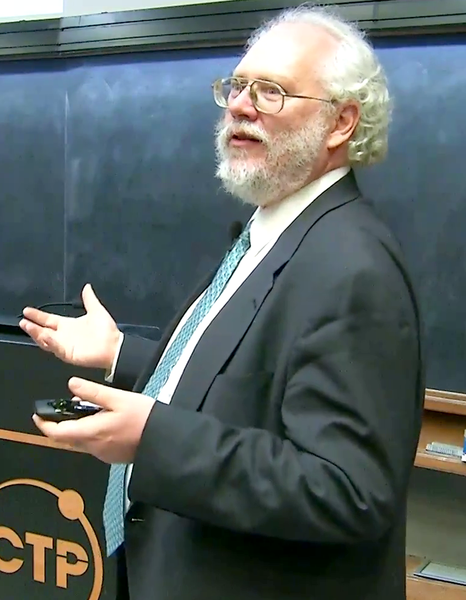
\includegraphics[width=0.3\textwidth]{Peter_Shor.png}
    \end{center}
    \vspace{-20pt}
    \caption{Peter Shor en la ceremonia de entrega de la medallla Dirac en 2017.}
    \vspace{-10pt}
\end{wrapfigure}

\par Shor comenzó su puesto en el MIT en 2003. Actualmente, es profesor Henry Adams Morss y Henry Adams Morss, Jr. de Matemáticas Aplicadas en el Departamento de Matemáticas del MIT. También está afiliado a CSAIL y al Centro de Física Teórica (CTP) del MIT.

\par El 1 de octubre de 2011, fue incluido en la Academia Estadounidense de las Artes y las Ciencias. Fue elegido miembro de ACM en 2019 ``por sus contribuciones a la computación cuántica, la teoría de la información y los algoritmos aleatorios". Fue elegido miembro de la Academia Nacional de Ciencias en 2002. En 2020, fue elegido miembro de la Academia Nacional de Ingeniería por sus contribuciones pioneras a la computación cuántica.

\par Peter Shor es conocido por su trabajo en computación cuántica, en particular por diseñar el algoritmo de Shor, un algoritmo cuántico para factorizar exponencialmente más rápido que el mejor algoritmo actualmente conocido que se ejecuta en una computadora clásica.

\section*{\center\itshape\large Algoritmo cu\'antico de Shor}

\par Desde 1900AC, se han venido empleando formas de criptografía; el propósito fundamental, de este campo, siempre ha consistido en encontrar un medio seguro de enviar mensajes.  En 1981 el físico teórico estadounidense Richard Feynman en el MIT propuso un modelo básico para un computadora cuática. Resulta común hoy en día, escuchar que la computadora cuántica podría romper el criptosistema de llave pública RSA. Sin embargo en la práctica aún se está un poco lejos de esa realidad.

\par Peter Shor, el matemático estadounidense mientras trabajaba en Bell Labs, New Jersey en 1995, formuló el ``Algoritmo de Shor". El algoritmo fue diseñado para la factorización de números enteros. Shor probó que una computadora cuántica cuando opera de manera óptima (ignorando el ruido y otra interferencia cuántica relacionada) podría romper con eficacia los esquemas criptográficos clásicos como el RSA. Un gran problema de factorización de enteros ha sido una importante limitación de la criptografía clásica, pero las computadoras cuánticas aprovecha el algoritmo de Shor para resolver este problema\textsuperscript{\textcolor{cyan}{\cite{2}}}.\\

\par Este algoritmo cuántico o como se le llama en la literatura, algoritmo de Shor, se puede enunciar de la siguiente forma:

\subsection*{\normalsize Algoritmo de Shor}

\begin{itemize}
    \item[] {\bfseries Entrada:} Un n\'umero compuesto $N$.
    \item[] {\bfseries Salida:} Un factor no trivial de $N$.
    \item[] {\bfseries Tiempo de ejecuci\'ion:} $O(log^3 N)$
    \item[] {\bfseries Procedimiento:}
    \begin{itemize}
        \item[1.] Primero se selecciona un entero positivo $m<n$, luego se calcula el $gcd(m,n)$ en tiempo polinomial usando el algoritmo Euclideano. Si el $gcd(m,n)\neq 1$, el problema fue resuelto, de lo contrario se procede al paso 2.
        \item[2.] Una computadora cuantica es usada para calcular el valor desconocido del per\'iodo $P$ de la secuencia $m\, mod\, n$, $m^2\, mod\, n$, $m^3\, mod\, n$, ..., $m^P\, mod\, n$, ....
        \item[3.] Si $P$ es impar, se regresa al paso 1 y, si es par, entonces $m^P-1=(m^{\frac{P}{2}}-1)(m^{\frac{P}{2}}+1)$ y se procede al paso 4.
        \item[4.] Si $m^{\frac{P}{2}}+1 \equiv 0 (mod\, n)$, se regresa al paso 1, de lo contrario se llega al paso 5.
        \item[5.] Finalmente se computa $d=gcd(m^{\frac{P}{2}}-1,n)$ mediante el algoritmo Euclideano y se resuelve el problema.
    \end{itemize}
\end{itemize}

\par Como se mencionaba al comienzo, el algoritmo Shor, pone en posición de jaque no solo a RSA sino a otras criptografías de llaves públicas. No obstante cabe señalar que hasta hoy en día solo se han podido factorizar en la práctica usando computadoras ``cuánticas” reales los números 15 y 21; las razones, se enumeran a continuación:
\begin{itemize}
    \item[1)] No se sabe ni se tiene un consenso mundial de cuál es la mejor forma de construir una computadora cuántica (fotones, trampas de iones, superconductores, etc..)
    \item[2)]  Resulta extremadamente difícil y costoso mantener en el tiempo un qubit así como hacer cambios en él que no produzcan errores.
\end{itemize}

\par Hasta ahora, muchos investigadores de la ciencia cuántica han intentado implementar el algoritmo de Shor con sistemas cuánticos; sin embargo, ninguno ha tenido éxito de forma escalable con más de unos pocos bits cuánticos.

\par Aunque no es menos cierto que en los últimos años, compañías como Google, IBM, así como los mega-proyectos del gobierno Chino encaminados al desarrollo de la computación cuántica; han tenido un avance como nunca antes visto; el genial artículo que publica Shor en el 1994 que viene a ser el comienzo de la computación cuántica como rama de investigación, se ha resistido fuertemente a ser llevado a la práctica. IBM líder mundial en este tema investigación asegura tener 1024 qubits para el 2023 y como contraste casi todos los trabajos teóricos relacionados con la llamada quantum-error-correction afirman: que para poder operar 1024 qubits se necesitan en realidad millones para que el resto se encargue de los errores.\\

\par La más conocida aplicación de un dispositivo de cómputo cuántico usando el algoritmo de Shor es la capacidad de romper cualquier sistema criptográfico basada en RSA. Esta aparente ventaja ha motivado a que especialmente en EE.UU y Europa el estudio de este algoritmo y la construcción de un ordenador cuántico sean apoyados
fuertemente con fondos gubernamentales, catalogando estas investigaciones como clasificadas. Es muy claro que de ninguna manera habrá a mediano plazo un gran mercado para este tipo de dispositivos que descompone en factores: ya que la misma existencia de tal máquina conducirá a la total desaparición del esquema RSA, pero permitirá el surgimiento de sistemas de encriptación con tecnologías substitutas como la criptografía cuántica. Tan solo el futuro lo dirá.

\section*{\center\itshape\large Alcance de los algoritmos cuánticos}

\par Con los algoritmos cuánticos, se define una nueva clase de complejidad cu\'antica: BQP por sus siglas bounded-error, quantum, polynomial, y representa aquellos problemas que pueden ser resueltos eficientemente por una computadora cu\'antica donde una peque\~na probabilidad de error es permitida\textsuperscript{\textcolor{cyan}{\cite{3}}}.

\begin{wrapfigure}{l}{0.3\textwidth}
    \vspace{-20pt}
    \begin{center}
        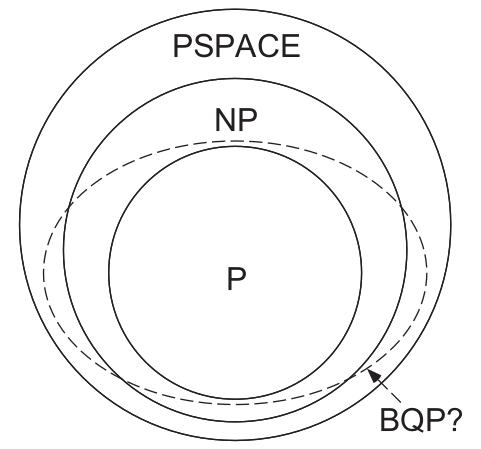
\includegraphics[width=0.28\textwidth]{diagrama.png}
    \end{center}
    \vspace{-20pt}
    \caption{Relacion entre las clases de complejidad.}
    \vspace{-10pt}
\end{wrapfigure}

\par Como se puede apreciar en la Figura 2, la clase BQP contiene a todos los problemas de tipo P y a unos cuantos de tipo NP, como el de la factorizaci\'on, gracias al algoritmo de Shor o el llamado problema del algoritmo discreto. Se cree que el resto de los problemas NP y NP-Completos caen fuera de la clase BQP, lo que significa que incluso un ordenador cu\'antico necesitar\'ia m\'as que un n\'umero polin\'omico de pasos para resolverlos.

\par Por otra parte, los problemas BQP podr\'ian desbordar la clase NP: las computadoras cu\'anticas podr\'ian resolver ciertos problemas en menos tiempo incluso del que invertir\'ia un ordenador com\'un en comprobar la soluci\'on. Hasta la fecha, sin embargo, no se conocen ejemplos convincentes de problemas de este tipo\textsuperscript{\textcolor{cyan}{\cite{4}}}.

\section*{\center\itshape\large Conclusiones}

\par Este documento ha sido capaz de simplificar e introducir a los lectores a la computaci\'on cu\'antica y espec\'ificamente el algoritmo de Shor. Se expuso de forma adecuada el contexto en el cual se cre\'o dicho algoritmo haciendo \'enfasis tamb\'ien en la historia de su desarrollador. Se proporcion\'o una definici\'on formal del mismo y un algoritmo completamente v\'alido para su correcto funcionamiento, dotando al lector de las herramientas necesarias para futuras investigaciones relacionadas con el tema; adem\'as de un panorama del alcance que est\'an teniendo los algoritmos cu\'anticos en la ciencia y en la actualidad, cumpliendo de esta forma los objetivos perseguidos con la presente investigaci\'on.

\newpage
\begin{thebibliography}{3}
    \bibitem{1} \href{https://math.mit.edu/~shor/}{\textcolor{cyan}{\underline{Pagina de Peter Shord en el MIT}}}.

    \bibitem{2} Chikodili Ugwuishiwu, Orji Ugochukwu, International Journal of Advanced Trends in Computer Science and Engineering. \emph{An overview of Quantum Cryptography and Shor's Algorithm}.

    \bibitem{3} Michael A. Nielsen y Isaac L. Chuang. \emph{Quantum Computation and Quantum Information}.

    \bibitem{4} Scott Aaronson, \emph{Los L\'imites de la Computaci\'on Cu\'antica}.
\end{thebibliography}

\end{document}
